\section{Adaptive Recommenders}
\label{sec:adaptive}

\emph{Adaptive Recommenders} (AR) is a technique for combining recommender systems
in an effort to answer two important questions.
Given that we wish to predict the relevance of an item to a user,
using many methods that consider disjoint data patterns,

\begin{enumerate*}
  \item What rating does each method predict?
  \item How accurate will each of these predictions be?
\end{enumerate*}

User modeling methods and recommender systems traditionally only care about the first question:
a single method is used to predict an unknown rating.
Modern aggregation techniques goes one step further, and combines many methods using a generic (often weighted) combination
(e.g. \cite{Bell2007b, Huang2002}).
However, we wish to make the aggregation \emph{adaptive},
so that the aggregation itself depends on which user and which item we are considering.

Formally, we define adaptive recommenders as \emph{adapting a set of recommender systems
with another complementary set of recommender systems} 
(see Figure \ref{fig:adaptiveusermodeling}).
The first set creates standard prediction scores, and answers the first question.
The second set predicts how accurate each method will be for the current user and item,
answering the second question.
The interesting bit is that AR can use recommender systems for both these tasks, as we shall soon see.
A system for adaptive recommenders is specified by a 6-tuple, 
$\mathrm{AR} = (I,U,R,F,M,A)$.

We have sets of $Users$ ($U$) and $Items$ ($I$), 
and a set of $Ratings$ ($R$): each user $u \in U$ can produce a rating $r \in R$ of an item $i \in I$.
Items can be just about anything: documents, websites, movies, events, or indeed, other users.
The ratings can be explicitly provided by users, for example by rating movies,
or they can be mined from existing data, for example by mining query logs.
We use the term "rating" loosely --- equivalent terms include \emph{relevance}, \emph{utility},
\emph{score} or \emph{connection strength}. In other words, this is a measure of what a user thinks of an item
in the current domain language. However, since \emph{rating} 
matches the data in our experiment, that is what we shall use.

The $Framework$ ($F$) variable specifies how the data is represented.
The two canonical ways of representing users, items and ratings are graphs and matrices 
(see \cite{Mirza2003}).
We shall use a matrix, where the first dimension corresponds to users, the second to items, and each populated cell is an explicit or implicit rating:

\begin{equation*}
 R_{u,i} =
 \begin{pmatrix}
  r_{1,1} & r_{1,2} & \cdots & r_{1,i} \\
  r_{2,1} & r_{2,2} & \cdots & r_{2,i} \\
  \vdots  & \vdots  & \ddots & \vdots  \\
  r_{u,1} & r_{u,2} & \cdots & r_{u,i}
 \end{pmatrix}.
\end{equation*}

As we wish to leverage disjoint data patterns, we have a set of modeling $Methods$, 
each with their own way of estimating unknown ratings. 
Each model $m \in M$ is used to compute independent and hopefully complimentary predictions.
In our case, these methods are recommender systems.

As demonstrated in 
\cite{Adomavicius2005, Pazzani2007, Schafer2007, Segaran2007},
there are many different recommendation algorithms,
that consider different aspects in the data: users, items and ratings, as well as 
sources such as intra-user connections in social networks or intra-item connections in information retrieval systems.
Examples of such recommender systems include Slope One predictions \cite{Lemire2005}, 
SVD factorization (e.g. \cite[p5]{Billsus}, \cite{Sun2005} and \cite{Bell2007}) and 
Nearest Neighbor weighted predictions \cite[p11]{Segaran2007}.
These methods predict unknown connections between users and items based on some pattern in the data,
for example user profile similarity, rating correlations or social connections.
As previously explained, to achieve the best possible combined result, we wish to use methods that look at disjoint patterns, 
i.e. complementary predictive parts of the data
(as described by \cite[p1]{Bell2007b}).

The $Adapters$ ($A$) part of our 6-tuple refers to the second level of user modeling methods.
In traditional prediction aggregation this is a simple linear function for combining the different predictions,
for example by pre-computing a set of weights, one for each method.
As found by \cite[p6]{Bell2007} the accuracy of the combined predictor is more dependent on the 
ability of the various predictors to expose different aspects of the data, than on 
the individual accuracy of each predictor.
Multiple prediction results are normally combined into a final singular result,
based on a generalized combination found by minimizing some error across all users.

With adaptive recommenders, the $Adapters$ are themselves user modeling methods.
However, instead of modeling users, we wish to model each recommender system.
More specifically, we wish to model the \emph{accuracy} of each recommender system.
Methods in this second layer are used to predict how accurate each of their corresponding basic recommenders will be.
It is these methods that will allow us to do adaptive aggregation based on the current user and item.
In other words, we have two distinct layers of user modeling 
(see Figure \ref{fig:adaptiveusermodeling}):

\begin{figure*}[!t]
  \center
  \def\layersep{2cm}
  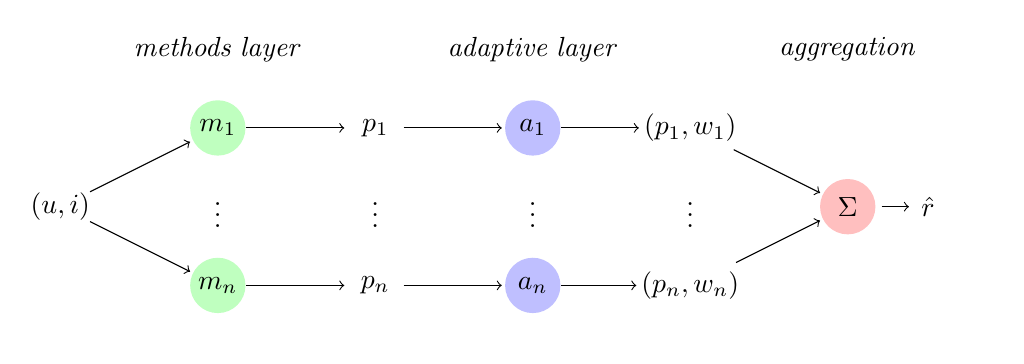
\begin{tikzpicture}[shorten >=1pt,->,draw=black, node distance=\layersep]

    \tikzstyle{every pin edge}=[<-,shorten <=2pt]
    \tikzstyle{node}=[circle,fill=black!25,minimum size=20pt,inner sep=0pt]
    \tikzstyle{input node}=[node, fill=green!25];
    \tikzstyle{output node}=[node, fill=red!25];
    \tikzstyle{hidden node}=[node, fill=blue!25];
    \tikzstyle{annot} = [text width=10em, text centered]
    \tikzstyle{txt}=[node,fill=white];
    
    \node[txt] (UI) at (0,-2) {$(u,i)$};  

    \node[input node] (I-1) at (\layersep,-1) {$m_1$};
    \node[txt]        (I-D) at (\layersep,-2) {$\vdots$};
    \node[input node] (I-N) at (\layersep,-3) {$m_n$};
    
    \node[txt] (P-1) at (\layersep*2, -1) {$p_1$};
    \node[txt] (P-D) at (\layersep*2, -2) {$\vdots$};
    \node[txt] (P-N) at (\layersep*2, -3) {$p_n$};

    \node[hidden node] (H-1) at (\layersep*3, -1) {$a_1$};    
    \node[txt]         (H-D) at (\layersep*3, -2) {$\vdots$};    
    \node[hidden node] (H-N) at (\layersep*3, -3) {$a_n$};    

    \node[txt] (R-1) at (\layersep*4, -1) {$(p_1,w_1)$};
    \node[txt] (R-D) at (\layersep*4, -2) {$\vdots$};
    \node[txt] (R-N) at (\layersep*4, -3) {$(p_n,w_n)$};
    
    % hidden helper node
    \node[txt] (HH)  at (\layersep*5,-1) {};

    % Draw the output layer node
    \node[output node,pin={[pin edge={->}]right:$\hat{r}$}] at (\layersep*5,-2) (O) {$\Sigma$};
    
    \path (UI) edge (I-1);
    \path (UI) edge (I-N);

    \path (I-1) edge (P-1);
    \path (I-N) edge (P-N);

    \path (P-1) edge (H-1);
    \path (P-N) edge (H-N);

    \path (H-1) edge (R-1);
    \path (H-N) edge (R-N);

    \path (R-1) edge (O);
    \path (R-N) edge (O);

    % Annotate the layers
    \node[annot,above of=I-1, node distance=1cm] {\emph{methods layer}};
    \node[annot,above of=H-1, node distance=1cm] {\emph{adaptive layer}};
    \node[annot,above of=HH,  node distance=1cm] {\emph{aggregation}};
  \end{tikzpicture}

  \vspace{1em}
  \caption[The Layers of Recommenders]{
    Layers of recommenders:
    The method layer consists of ordinary modeling methods,
    each predicting the rating between a user and an item.
    This produces a set of predicted ratings ($p$).
    The adaptive layer estimates how well each modeling method
    will perform for the current user and item,
    and weighs the predictions accordingly.
    This produces a set of predictions and weights [$(p,w)$].
    The aggregation weighs the predictions into a final score $\hat{r}$.  
  }
  \label{fig:adaptiveusermodeling}
\end{figure*}


\subsection{Adaptive Aggregation}

To perform adaptive aggregation, we need the $Adapters$ to be actual recommender systems.
The simplest generalized way of prediction aggregation is to take the average of all predictions made
by the different methods (e.g. \cite[p3]{Aslam2001}).
However, many aggregators attempt to weigh each method differently (e.g. \cite{Claypool1999}):

\begin{eqnarray*}
  \hat{r}_{u,i} = \sum_{m \in M} w_{m} \times p(m,u,i).
\end{eqnarray*}

Here, $w_m$ is the weight applied to modeling method $m$. 
These weights fall in the range $[0,1]$ and sum up to $1$.
The weights can be estimated through different machine learning methods.
However, as discussed in Section \ref{sec:intro},
this is still a generalized result, averaged across every prediction.
The system assumes that the best average result is the best result for each individual user and item.
Even with method-specific weights we are still hindered by the latent subjectivity problem.

In order to leverage as many patterns as possible while sidestepping the latent subjectivity,
we need \emph{adaptive weights} that are computed specifically for each combination of a user and an item.
However, if we wish each weight to be combination-specific, pre-computing each weight for each method becomes unfeasible
--- we would have to compute a weight for each method for each possible rating.
In other words, these adaptive weights also have to be estimated, just as the ratings themselves:

\begin{eqnarray*}
  \hat{r}_{u,i} = \sum_{m \in M} p_{w}(m,u,i) \times p_{r}(m,u,i).
\end{eqnarray*}

Here, $p_w(m,u,i)$ is the predicted optimal weight for method $m$ when applied to user $u$ and item $i$.
We have reduced our mission of adaptive prediction aggregation to creating this function.

We wish to use standard recommender systems for predicting optimal adaptive weights.
To do this, we need to create a matrix (or graph)
that stores known values of how accurate some of the rating predictions will be.

This can be done my modeling the errors of each method.
By modeling the errors with standard recommender systems,
we can in turn predict errors for untested combinations.
If we predict the error of a recommender system for a user and an item,
we have also predicted its accuracy.
To achieve this, we can create an \emph{error matrix}:

\begin{equation*}
 E_{u,i} =
 \begin{pmatrix}
    e_{1,1} & e_{1,2} & \cdots & e_{1,i} \\
    e_{2,1} & e_{2,2} & \cdots & e_{2,i} \\
    \vdots  & \vdots  & \ddots & \vdots  \\
    e_{u,1} & e_{u,2} & \cdots & e_{u,i}
 \end{pmatrix}
\end{equation*}

Creating an error matrix for each modeling method is quite simple:
by splitting the ratings data in two,
the first set can be used for the actual training, and the second
can be used to populate each error matrix.

Each standard modeling method gets an error matrix where some cells have values:
each value corresponds to the prediction error for a combination of a user and an item.
Each modeling method is trained with a part of the ratings data.
The error matrix is populated from the rest of the data,
by computing the error of each known rating the method was not trained for:

\begin{eqnarray*}
  \forall (u,i,r) \in (d_e - d_m): E(m)_{u,i} = |r - p(m,u,i)|.
\end{eqnarray*}

Here, $D$ is the current dataset, and
$d_m$ and $d_e$ are subsets of $D$.
$m$ is a modeling method trained with the subset $d_m$.
To populate the error matrix for this method,
we take each rating which have not been used to train the method
and calculate the error of the method on this combination.
The result is a sparse error matrix
we can use to predict unknown errors.
Notice how similar this matrix is to the previously introduced ratings matrix.
This similarity is what will allow us using standard recommender systems
to perform adaptive aggregation.


\subsection{Modeling Phase}

Whenever we wish to train a new modeling method,
\emph{the modeling phase}, we apply the following algorithm:

\begin{enumerate*}
  \item Split the ratings data into two sets for training and error estimation.
  \item Train the modeling method in its specific way with the first training set.
  \item Use the error estimation data set to create the error matrix.
  \item Train an error model based on the error matrix.
\end{enumerate*}

Constructing the subsets of the available data is a common task in ensemble learning
\cite[p7]{Polikar2006}.
We use \emph{bootstrap aggregation}, also known as \emph{bagging} (introduced by \cite{Breiman1996}).
Originally, bagging is used by ensemble learning classification methods, where multiple classifiers are 
trained by uniformly sampling a subset of the available training data. 
Each model is then trained on one of these subsets, and the models are aggregated by averaging their individual predictions.

Bagging suits our needs perfectly, for a few reasons: First, the method helps create disjoint predictors, 
since each predictor is only trained (or specialized for) a subset of the available data.
Second, it allows us to easily train the underlying modeling methods without any complex partitioning of the data.
Our partitioning strategy is now clear:

The error models are trained using standard recommender systems.
After all, the mission is the same:
we have two dimensions, with a sparse set of known connections,
and wish to predict unknown connections from this data.
The result is a set of modeling methods
that can predict the error of a recommender system
when its used on a particular user and item combination.

What will happen when we train a recommender system with the error matrix?
First of all, the errors will be on the same scale as the initial ratings.
Second, just as the ratings matrix will include noise (ratings that
do not contribute to any underlying pattern), this will be 
true for the error matrix as well.

For example, one method might have a large error for a particular user and item combination,
yet still work well for both these elements. 
Luckily, this is 
just the kind of noise recommender systems are good at pruning away.
What we are interested in are situations where a method
has stable and significant errors for many ratings from a user,
or many ratings of an item.
In this case, there is a pattern where this method does not 
work well for the element in question.
This is exactly the kind of pattern recommender systems are good at identifying.

In other words, the same capabilities that makes recommender systems work well
on the ratings matrix, will also make them work well on the error matrix.
The properties we need for predicting ratings
are the same as those needed to predict accuracy.

Of course, some recommender systems will work better than others for the adaptive layer.
Most often we are seeking global patterns in the data.
We are looking for groups of users or items (or both) that suite some 
recommenders especially well, or that some recommenders will not work for.
SVD-based recommenders is one type of RS that can be used for this purpose.
By reducing the method-error space into an "error category space",
we can identify how well a set of groups suite each available method.
We will get back to this when testing the performance
of our approach in Section \ref{sec:results}.


\subsection{Prediction Phase}

When we have an error model for each modeling method, 
we can use these errors to estimate each weight.
Whenever we wish to create an adaptive aggregate prediction,
\emph{the prediction phase},
we apply the following algorithm:

\begin{enumerate*}
  \item Collect predictions from each modeling method for $(u,i)$.
  \item Collect estimated errors for each method for $(u,i)$.
  \item Compute weights for each method based on their relative predicted errors.
  \item Sum the weighted predictions to get the adaptively predicted rating.
\end{enumerate*}

The next section will explain these steps in detail.
We can now express the prediction phase of adaptive recommenders as an equation.
Each rating/relevance prediction is weighted by its predicted accuracy,
conditioned on the current user and item,
as seen in Equation \ref{eq:adaptive}.

\begin{figure*}[!t]
\normalsize
\begin{eqnarray}
  \label{eq:adaptive}
  \hat{r}_{u,i} = \sum_{(m_{e}, m_{r}) \in M} (1 - 
  \frac{
    p(m_{e},u,i)
  }{
    error(u,i)
  }) \times p(m_{r},u,i)
  \quad
  \text{where}
  \quad
  error(u,i) = \sum_{m_e \in M} p(m_e,u,i) 
\end{eqnarray}
\hrulefill
\vspace*{4pt}
\end{figure*}

In Equation \ref{eq:adaptive}, each recommender method has two corresponding models:
$m_r$ is the ratings model, used to predict ratings, and
$m_e$ is the error model, used to predict errors.
$p(m,u,i)$ is the prediction of the model $m$ (a recommender system)
for the relevance of item $i$ to user $u$.
Each method is weighted by its predicted accuracy.
The weights are computed by taking the opposite
of each methods predicted error.
The errors are normalized across each user and item by $errors(u,i)$,
which is the sum of the errors of each method for the current combination.
This gives us weights in the range $[0,1]$ ensuring
final rating predictions on the same scale as that returned by the basic recommenders.

Notice that the \emph{only} difference between $m_e$ and $m_r$ is how they are created.
$m_r$ is trained with the standard ratings matrix, and $m_e$ is trained using the error matrix.
This means we can use \emph{any} standard recommender system to perform adaptive aggregation.
Hence, the name \emph{adaptive recommenders}:
a set of secondary recommenders is used to adapt a set of standard
recommenders to each user and item.

It is also important to note that the types of recommenders used for the adaptive layer
is independent of the basic recommenders.
Each adaptive recommender need only predicted ratings from each basic recommender,
and does not care which algorithm it employs.
When making predictions, the calculations in the methods layer and adaptive layer
are independent of each other, as both use pre-computed models:
the method layer use the ratings matrix, or their own models
created during training, while the adaptive layers use the error matrices for each
basic method.

The result of this is a system that does not only aggregate a number of predictions for each unknown
combination of users and items,
but that also combines these methods based on how accurate each prediction is likely to be.
Now that we have our model, it is time to see how it performs.


